%% Author_tex.tex
%% V1.0
%% 2012/13/12
%% developed by Techset
%%
%% This file describes the coding for rsproca.cls

\documentclass{rsproca}%%%%where rsproca is the template name

\RequirePackage{fix-cm}
\usepackage{caption}
\usepackage{subcaption}

%%%% *** Do not adjust lengths that control margins, column widths, etc. ***

%%%%%%%%%%% Defining Enunciations  %%%%%%%%%%%
\newtheorem{theorem}{\bf Theorem}[section]
\newtheorem{condition}{\bf Condition}[section]
\newtheorem{corollary}{\bf Corollary}[section]
%%%%%%%%%%%%%%%%%%%%%%%%%%%%%%%%%%%%%%%%%%%%%%%

\jname{rspa}
\Journal{Proc R Soc A\ }

\captionsetup{justification=centering}
\begin{document}

%%%% Article title to be placed here
\title{Numerical Solutions of Ideal Quantum Gas Dynamical Flows Governed by Semi-classical Ellipsoidal-Statistical Distribution}

\author{%%%% Author details
Jaw-Yen Yang$^{1,2}$, Chih-Yuan Yan$^{1}$, Manuel Diaz$^{1}$, Juan-Chen Huang$^{3}$, Zhihui Li$^{4}$ and Hanxin Zhang$^{4}$}

%%%%%%%%% Insert author address here
\address{$^{1}$Institute of Applied Mechanics, National Taiwan University, Taipei 10764, TAIWAN\\
$^{2}$Center for Advanced Study in Theoretical Science, National Taiwan University, Taipei 10764, TAIWAN\\
$^{3}$Department of Merchant Marine, National Taiwan Ocean University, Taipei 10764, TAIWAN\\
$^{4}$China Aerodynamics Research and Development Center, Mianyang, 621000, CHINA}


%%%% Subject entries to be placed here %%%%
\subject{Semi-classical Boltzmann equation, Semi-classical Ellipsoidal Statistical Model, Kinetic Numerical Method, Quantum Gas Dynamical Flows}

%%%% Keyword entries to be placed here %%%%
\keywords{Semi-classical Boltzmann equation, Ellipsoidal statistical Bhatnagar-Gross-Krook, Total variation diminishing (TVD), Discrete ordinate method, Two-dimensional Riemann problems}

%%%% Insert corresponding author and its email address}
\corres{Jaw-Yen Yang\\
\email{yangjy@iam.ntu.edu.tw}}

%%%% Abstract text to be placed here %%%%%%%%%%%%
\begin{abstract}
The ideal quantum gas dynamics as manifested by the semiclassical ellipsoidal statistical equilibrium distribution as derived in \cite{Wu2012} is numerically studied for particles of three statistics.  This anisotropic ellipsoidal statistical (ES) equilibrium distribution was derived through maximum entropy principle and conserves the mass, momentum and energy but differs from the standard Fermi-Dirac or Bose-Einstein distribution. The present numerical method combines the discrete velocity (or momentum) ordinate method in momentum space and high resolution shock capturing method in physical space.   A decoding procedure to obtain the necessary parameters for determining the ellipsoidal statistic distribution is also devised.  Computations of two-dimensional Riemann problems are presented and various contours of the quantities unique to this ES model are illustrated.  The main flow features such as shock wave, expansion wave and slip line and their complex nonlinear interaction are depicted and are found to be consistent with existing calculations for classical gas.
\end{abstract}
%%%%%%%%%%%%%%%%%%%%%%%%%%%

%%%%%%%%%% Insert the texts which can accomdate on firstpage in the tag "fmtext" %%%%%

%\begin{fmtext}
%\section{Introduction}
%This is just an example
%\end{fmtext}

%%%%%%%%%%%%%%% End of first page %%%%%%%%%%%%%%%%%%%%%

\maketitle

\section{Introduction}
\label{sec:1}

The kinetic Boltzmann equation has been commonly used to describe various transport phenomena in classical dilute gases covering wide range of flow parameters such as Reynolds number, Mach number and Knudsen number.   Analogous to the classical Boltzmann equation, a semiclassical Boltzmann equation, which generalizing the collision term to treat collision of particles of quantum statistics, has been developed by Uehling and Uhlenbeck \cite{PhysRev.43.552}, see \cite{KadanoffBaym,PhysRev.43.552}.
In recent years, due to the rapid advancements of nanotechnology, the device or structure characteristic length scales become comparable to the mean free path and the wavelength of energy and information carriers (mainly electrons, photons, phonons, and molecules), some of the classical continuum transport laws are no longer applicable.   It is generally believed that the microscopic description of Boltzmann equation (classical or semiclassical) is adequate to treat transport phenomena in the mesoscale range.  Hydrodynamic behaviour of quantum gases has been the subject of some prominent researches, see \cite{nikuni98,PhysRev.40.749,PhysRevB.35.7959}, and the application of quantum Boltzmann hydrodynamic equations have been implemented in the analysis of electron flows in quantum semiconductor devices, see \cite{Gardner1994,PhysRevB.39.9536,Woolard5146296}.  Besides, due to the different types of carriers may involve simultaneously in a single problem, it is desirable to have a method that can allow one to treat them in a unified and parallel manner.   With the semiclassical Boltzmann equation, it is possible to describe adequately the mesoscale transport of particles of arbitrary statistics.

The main difficulty encountered in solving the semiclassical Boltzmann equation is similar to that encountered in the classical counterpart and is mainly due to the complicated integral nature of its collision term.  The relaxation time approximation proposed by Bhatnagar, Gross and Krook (BGK) \cite{PhysRev.94.511} for the classical Boltzmann equation provides a simpler form of collision term and retains the principal effects of particle collisions and enables more tractable solution methods.  The relaxation time approximation is quite general and is applicable to the semiclassical Boltzmann equation.   The only change is that the equilibrium Maxwell-Boltzmann distribution in the classical case is replaced by the Bose-Einstein or Fermi-Dirac distribution depending on the types of carrier particles considered.  Indeed, the semiclassical Boltzmann-BGK equation has been widely used in electron carrier transport in semiconductor \cite{Lundstrom:2000,Fatemi1993209,Carrillo2003498,Majorana2001649,Carrillo2003JCEL,Carrillo2003b,Markowich2002,Pattamatta2009,Scaldaferri2007} and phonon energy transport in thermoelectric materials \cite{mit2005nanoscale}.   The main shortcoming of the classical BGK model is that the Prandtl number is equal to one while it is $2/3$ from the full Boltzmann equation.  In order to improve the classical Boltzmann-BGK model equation which does not produce correct Prandtl numbers, a new kinetic model called the ellipsoidal statistical model was proposed by Holway \cite{Holway1966}.  Analogously, a semiclassical ellipsoidal statistical kinetic model for quantum gases in the normal phase has been recently developed by Wu, Meng and Zhang \cite{Wu2012}.  This new model mimics the classical ellipsoidal statistical (ES) model of Holway \cite{Holway1966} and was derived by maximizing the corresponding entropy function under some constraints.   It possesses all the desirable features of a kinetic model and yields a correct Prandtl number for Fermi gases.   In the semiclassical Boltzmann-BGK equation, if the equilibrium Bose-Einstein or Fermi-Dirac distribution is replaced by the semiclassical ES distribution, then one has the semiclassical Boltzmann-ES-BGK equation \cite{Wu2012}.

Theoretically, the Chapman-Enskog expansion method is usually applied to the full Boltzmann or model Boltzmann equation (classical or semiclassical) to yield sets of governing hydrodynamic transport equations, such as Euler, Navier-Stokes and Burnett equations which are respectively the zeroth order, first order and second order expansions in the parameter Knudsen number,  see \cite{Cowling1970}.   The zeroth order solution yields the equilibrium distribution in phase space and the Euler equations in physical space and governs the ideal gas dynamics.  The semiclassical ES equilibrium distribution is the zeroth order solution of the semiclassical Boltzmann-ES-BGK equation.  It is the main objective of this work to investigate the ideal gas dynamics as governed by the semiclassical ellipsoidal statistical equilibrium distribution as it has not been well explored before.   The main numerical method adopted is a direct solver in phase space for the semiclassical ellipsoidal statistical equilibrium distribution function.  The direct solver consists of two methods; one is the discrete ordinate method and the other the high resolution shock-capturing methods.   In the classical rarefied gas flow computation, the implementation of discrete ordinate method to nonlinear model Boltzmann equations has been developed by Yang and Huang \cite{Yang1995323}.  Such a direct method will allow one to examine the same physical flow problems but with different gas of particles.   Also, if the classical limit situations of the same flow problem are considered, then one expect to obtain similar or identical flow structures for the three statistics.   It is noted that even with the classical Maxwell-Boltzmann statistics, the present formulation includes the fugacity which is not seen in the original Boltzmann-BGK equation \cite{PhysRev.94.511} and most other existing works based on it.  Computer simulations of several two-dimensional Riemann problems in gas flows of arbitrary statistics are shown to illustrate the complex nonlinear wave manifestation of ideal quantum gas dynamics as governed by the semiclassical ES equilibrium distribution.

% L. Wu, J. Meng and Y. Zhang, Kinetic modelling of the quantum gases in the normal phase, Proc. R. Soc. A, 2012, doi: 10.1098/rspa.2011.0673.

The present paper is organized as follows.  Elements of semiclassical Boltzmann-ES-BGK equation is briefly described in Section \ref{sec:2}. Its relation with hydrodynamic equations is outlined. In Section \ref{sec:3}, governing equations in two space dimensions and their non-dimensional forms are detailed. In Section \ref{sec:4}, the present direct solution method in phase space is described.   The implementation of the discrete ordinate method and total variation diminishing schemes and the numerical quadrature to evaluate the macroscopic properties are detailed.   A decoding procedure to determine the key parameters for determining the equilibrium ES distribution is given.  In Section \ref{results}, numerical experiments of two-dimensional semiclassical Riemann problems of ideal gas dynamical flows are presented to illustrate the present method as well as the flow physics. Finally, concluding remarks will be given in Section \ref{remarks}.

\section{Semiclassical Boltzmann-ES-BGK Equation}
\label{sec:2}
In this section, the elements of semiclassical Boltzmann kinetic equation are briefly described.   Following \cite{PhysRev.43.552,KadanoffBaym}, we consider the extension of the Boltzmann equation to quantum systems due to Uehling and Uhlenbeck  in which they took the Pauli exclusion principle into account.
%%
\begin{equation}
\left(\frac{\partial f}{\partial t}+\frac{\bf p}{m}\cdot {\bf\nabla }_x-{\bf \nabla}_{\bf x} U({\bf x},t)\cdot {\bf\nabla }_{\bf p}\right)f\left({\bf p},{\bf x},t\right)=\left(\frac{\delta f}{\delta t}\right)^{UU}_{coll.}
\end{equation}
where $m$ is the particle mass, $U$ is the mean field potential and $f(\vec p, \vec x, t)$ is the distribution function
which represents the average density of particles with momentum $\vec p$ at the space-time point $\vec x, t$. The $(\delta f
/\delta t)_{coll.}$ denotes the collision term and according to Uehling and Uhlenbeck \cite{PhysRev.43.552}, it takes the form,
\begin{align}
(\frac{\delta f} {\delta t})^{UU}_{coll.} &= \int d {\bf p} \int d\Omega
K({\bf p}, {\bf q}, \Omega) \{ [ 1+ \theta f({\bf p}, t)][1+ \theta f({\bf q})]f({\bf p}^*, t)f({\bf q}^*, t) \nonumber \\
&- [ 1+ \theta f({\bf p}^*, t)][1+ \theta f({\bf q}^*)]f({\bf p}, t)f({\bf q}, t) \},
\end{align}
where $K({\bf p}, {\bf q}, \Omega)$ denotes the collision kernel and $\Omega$ is the solid angle and $\theta$ is a parameter which specifies the type of particle statistics.   Here, for $\theta=+1$, Bose-Einstein particles are considered, for $\theta=-1$, Fermi-Dirac particles, and for $\theta=0$, the Maxwell-Boltzmann classical particles are considered.  It is well known that the collision integral of the semiclassical Boltzmann equation will automatically vanish when the gas distribution function is in equilibrium and the equilibrium distribution function for general statistics can be expressed as
\begin{equation}
f^{eq}\left({\bf p},{\bf x},t\right) =\frac{1}{z^{-1}\,exp\left\{{\left[{\bf p}-m\,{\bf u}({\bf x},t) \right]}^2/2mk_BT({\bf x},t)\right\} -\theta }
\label{eq:Semiclassical_equilibrium_PDF}
\end{equation}
where $ {\bf u}({\bf x},t)$ is the, mean velocity, $T({\bf x},t)$ is temperature, $k_B$ is the Boltzmann constant and $z\left({\bf x},t\right)= exp\left({\mu ({\bf x},t)/k_BT({\bf x},t)}\right)$ is the fugacity, where $\mu$ is the chemical potential.  In (\ref{eq:Semiclassical_equilibrium_PDF}), again, \(\theta=-1\), denotes the Fermi-Dirac statistics, \(\theta=+1\), the Bose-Einstein statistics and \(\theta=0\) denotes the Maxwell-Boltzmann statistics.
To avoid the mathematical difficulty caused by the nonlinear integral collision term, the relaxation time approximation of Bhatnagar, Gross and Krook (BGK) is generally applied to replace the collision term of Uehling and Uhlenbeck, thus the semiclassical Boltzmann-BGK equation reads
\begin{equation}
\left(\frac{\partial f}{\partial t}+\frac{\bf p}{m}\cdot {\bf\nabla }_x-{\bf \nabla}_{\bf x} U({\bf x},t)\cdot {\bf\nabla }_{\bf p}\right)f\left({\bf p},{\bf x},t\right) =\left(\frac{\delta f}{\delta t}\right)_{coll.}= -\ \frac{f-f^{eq}}{\tau }
\end{equation}
where $\tau$ is the relaxation time and needs to be specified for each carrier scattering and $f^{eq}$ is given by Eq. (\ref{eq:Semiclassical_equilibrium_PDF}). Inspired by the classical ES kinetic model \cite{Holway1966} and using the maximum entropy principle, a new kinetic model equation has been proposed for dilute quantum gases in the normal phase \cite{Wu2012}.  This semiclassical ellipsoidal statistical (ES) kinetic model equation preserves the main properties of the semiclassical Boltzmann equation, including conservation of mass, momentum and energy, the entropy dissipation property and the rotational invariance.   It also can provide correct Prandtl numbers.   This semiclaasical Boltzmann-ES-BGK equation can be expressed as
\begin{equation}
\left(\frac{\partial f}{\partial t}+\frac{\bf p}{m}\cdot {\bf\nabla }_x-{\bf \nabla}_{\bf x} U({\bf x},t)\cdot {\bf\nabla }_{\bf p}\right)f\left({\bf p},{\bf x},t\right) = -\ \frac{f-f^{ES}}{\tau }
\label{eq:semiclassical_B_ESBGK}
\end{equation}
where $f^{ES}$ is an anisotropic reference equilibrium distribution function given by
\begin{equation}
f^{ES}\left({\bf p},{\bf x},t\right) =\frac{1}{z^{-1}\,exp\left\{{\left[ \frac{1}{2} \lambda_{\alpha \beta}^{-1} C_{\alpha} C_{\beta} \right]} \right\} -\theta }
\label{eq:semiclassical_ES_equilibrium_pdf}
\end{equation}
In Eq. (\ref{eq:semiclassical_ES_equilibrium_pdf}), $\lambda_{\alpha \beta}$ is a matrix and $\lambda_{\alpha \beta}^{-1}$ is its inverse, and $C_{\alpha} = \frac{p_{\alpha}}{m} - u_{\alpha}$ are the components of the thermal velocity.
The reference equilibrium distribution function $f^{ES}$ is derived by the maximum entropy principle under some constraints that the mass, momentum and energy are conserved and the following relations are satisfied,
\begin{subequations}
\begin{align}
n\left({\bf x},t\right) &= \int{\frac{\ d{\bf p}}{h^D}}\,f^{ES} \left({\bf p},{\bf x}, t\right), \\
\vec u \left({\bf x},t\right) &= \frac{1}{n(\bf x, t)}\int{\frac{\ d{\bf p}}{h^D}\,\frac{\bf p}{m}}\,f^{ES}\left({\bf p},{\bf x}, t\right), \\
W_{\alpha \beta} \left({\bf x},t\right) &= \int{\frac{\ d{\bf p}}{h^D}\,m C_{\alpha} C_{\beta} \,f^{ES} \left({\bf p},{\bf x}, t\right)}
\end{align}
\end{subequations}
where $D$ is the dimension of momentum space. and $W_{\alpha \alpha} = P_{\alpha \alpha}$ is required for the conservation of energy.

In principle, after solving the semiclassical Boltzmann-ES-BGK equation for the (non-equilibrium) distribution function $f$, all the macroscopic dynamic variables of interest such as number density, momentum density and energy density are low order moments of the distribution function and are defined by:
\begin{subequations}
\begin{align}
n\left({\bf x},t\right) &= \int{\frac{\ d{\bf p}}{h^D}}\,f\left({\bf p},{\bf x}, t\right), \\
\vec u \left({\bf x},t\right) &= \frac{1}{n(\bf x, t)}\int{\frac{\ d{\bf p}}{h^D}\,\frac{\bf p}{m}}\,f\left({\bf p},{\bf x}, t\right), \\
{\epsilon}\left({\bf x},t\right) &= \int{\frac{\ d{\bf p}}{h^D}\,\frac{{\bf p}^2}{2m}}\,f\left({\bf p},{\bf x}, t\right).
\end{align}
\end{subequations}
Other higher-order moments such as pressure tensor $P_{\alpha \beta}$ and the heat flux vector $Q_{\alpha}({\bf x},t)$ can also be defined accordingly as
\begin{align}
P_{\alpha \beta}({\bf x},t) &= \int{\frac{d{\bf p}}{h^D}(\frac{p_{\alpha}}{m}-u_{\alpha})(\frac{p_{\beta}}{m}-u_{\beta})\,f\,({\bf p},{\bf x},t)}, \\
Q_{\alpha}({\bf x},t) &= \int{\frac{d{\bf p}}{h^D}\frac{({\bf p}-m{\bf u})^2}{2m}(\frac{p_{\alpha}}{m}-u_{\alpha})\,f\,({\bf p},{\bf x},t)}.
\label{stressflux}
\end{align}
Lastly, to determine the semiclassical ellipsoidal statistical distribution $f^{ES}$, one usually needs to calculate $z$ and the matrix $\lambda_{\alpha \beta}$ simultaneously through
\begin{align}
&(\frac{m}{h})^D \sqrt{ ||2 \pi \lambda_{\alpha \beta}|| } \mathcal{Q}_{D/2}(z)= \frac{\rho}{m}, \\
&(\frac{m}{h})^D \sqrt{ ||2 \pi \lambda_{\alpha \beta}|| } \mathcal{Q}_{D/2 +1}(z) \lambda_{\alpha \beta} = \frac{W_{\alpha \beta}}{m},
\end{align}
where $||\cdot ||$ denotes the determinant of a matrix.   To obtain the $W_{\alpha \beta}$ to completely determine $f^{ES}$ and require that $W_{\alpha \alpha}=P_{\alpha \alpha}$ to insure conservation of energy, a natural choice leading to rotational invariance of the kinetic model equation is (Holway 1966)
\begin{equation}
W_{\alpha \beta}({\bf x},t) = (1 - b) p \delta_{\alpha \beta} + b P_{\alpha \beta}.
\end{equation}
where $p$ is the hydrodynamic pressure defined as the average of the diagonal components of the pressure tensor $P_{\alpha \beta}$, i.e., $p = P_{\alpha \alpha}/D$, and $b$ is a parameter.  Requiring $W_{\alpha \beta}$ to be positive definite, the parameter $b$ satisfies
\begin{align}
-\frac{1}{D-1} \le b < 1
\end{align}
for $D=2$ and $D=3$.

The conservation laws of macroscopic properties can be obtained by multiplying Eq. (\ref{eq:semiclassical_B_ESBGK}) respectively by 1, ${\bf p}$ and \({\bf p}^2/2m\)\, and integrating the resulting equations over all ${\bf p}$.  Consequently, the integrals of the collision terms in all three cases vanish automatically resulting in the conservation laws in differential equations form for the conserved macroscopic quantities i.e., number density \(n({\bf x},t)\), momentum density \(m n {\bf u}({\bf x},t)\), and energy density \(\epsilon({\bf x},t)\) as follow:

\begin{subequations}
\begin{align}
\frac{\partial n\left({\bf x},t\right)}{\partial t}&+{\bf \nabla }_x\cdot{\bf j}\left({\bf x},t\right)=0, \\
\frac{\partial m\/{\bf j}\left({\bf x},t\right)}{\partial t}&+{\bf \nabla }_x\cdot\int{\frac{d{\bf p}}{h^3}}\,{\bf p}\,\frac{\bf p}{m}f\left({\bf p},{\bf x},t\right)= -n({\bf x},t){\bf \nabla}_{\bf x}U({\bf x},t), \\
\frac{\partial \epsilon \left({\bf x},t\right)}{\partial t}&+{\bf \nabla }_x\cdot\int{\frac{d\bf p}{h^3}}\,\frac{\bf p}{m}\,\frac{{\bf p}^2}{2m}f\left({\bf p},{\bf x},t\right)=-{\bf j}({\bf x},t)\cdot{\bf \nabla}_{\bf x}U({\bf x},t).
\end{align}
\label{eq:semiclassical_ES_Euler}
\end{subequations}

In this work, we will focus our effort on the case of {\em semiclassical ES Euler} limit in which the particle distribution function is always in reference equilibrium, i.e., $f=f^{ES}$ and the collision term of Eq. (\ref{eq:semiclassical_B_ESBGK}) vanishes automatically and the set of governing equations, Eqs. (\ref{eq:semiclassical_ES_Euler}) will be termed semiclassical ellipsoidal statistical (ES) Euler equations in order to distinguish it from the semiclassical Euler equations as governed by $f=f^{eq}$.  It is noted that $f^{ES}$ is not isotropic and has quantities like $W_{\alpha \beta}$ and is quite different from $f^{eq}$, the standard Bose-Einstein and Fermi-Dirac distributions, thus it is worth some detailed study to explore the gas dynamical flow features inherent in this peculiar equilibrium distribution before we take on the non-equilibrium gas flows as governed by semiclassical Boltzmann-ES-BGK equation, i.e., Eq. (\ref{eq:semiclassical_B_ESBGK}). In the later section, we will present the comparison of results with these two semiclassical Euler solutions.  In recent years, notable numerical methods to describe the ideal quantum gas flows have been developed, see \cite{1272832,Shi20089389,Jaw-YenYang05082006}.

\section{Governing Equations in Two Space Dimensions}
\label{sec:3}
Here, we give detailed description of the theory and governing equation in two space dimensions.  Without losing generality, we also neglect the influence of externally applied field \(U({\bf x},t)\).  It is noted that quantum statistics of ideal gases in two dimensions has striking features such as the specific heat for an ideal gas of Fermi particles is identical with that for an ideal Bose gas \cite{May1964}. The general method in three space dimensions can also be similarly formulated.   When $f=f^{ES}$, the semiclassical Boltzmann-ES-BGK equation in two space dimensions can be expressed as
%%
\begin{align}
\frac{\partial f^{ES}({\upsilon}_x,{\upsilon}_y, x, y, t)}{\partial t} + {\upsilon}_x\,\frac{\partial f^{ES}({\upsilon}_x,{\upsilon}_y, x, y, t)}{\partial x } + {\upsilon}_y\,\frac{\partial f^{ES}({\upsilon}_x,{\upsilon}_y, x, y, t)} {\partial y} =0,
\label{eq:normalized_B_ES_BGK}
\end{align}
%%
with ${\upsilon}_x$ and ${\upsilon}_y$ as particle velocities.   The macroscopic properties are the various moments of $f^{ES}({\upsilon}_x,{\upsilon}_y,x,y,t)$,
\begin{subequations}
\begin{align}
\rho (x,y,t) 			&= \int \frac{ d p_x}{h} \frac{ d p_y}{h} \, f^{ES}(p_x, p_y, x, y, t), \\
u_x (x,y,t) 			&= \frac{1}{\rho} \int 	 \frac{ d p_x}{h} \, \frac{ d p_y}{h}  p_x \, f^{ES}(p_x, p_y, x, y, t), \\
u_y (x,y,t) 			&= \frac{1}{\rho} \int 	 \frac{ d p_x}{h} \, \frac{ d p_y}{h}  p_y \, f^{ES}(p_x, p_y, x, y, t), \\
\epsilon (x,y,t) 	&= \int \frac{ d p_x}{h} \frac{ d p_y}{h} \, \frac{(p_x^2 + p_y^2)}{2m} \, f^{ES}(p_x, p_y, x, y, t).
\end{align}
\end{subequations}
Additional information from $f^{ES}$ can also be defined accordingly to
\begin{subequations}
\begin{align}
W_{x x}(x,y,t)	&=	\int \frac{ d p_x}{h} \frac{ d p_y}{h} \, (\frac{p_x}{m}-u_x)(\frac{p_x}{m}-u_x)\,f^{ES}(p_x, p_y, x, y, t), \\
W_{x y}(x,y,t)	&=	\int \frac{ d p_x}{h} \frac{ d p_y}{h} \, (\frac{p_x}{m}-u_x)(\frac{p_y}{m}-u_y)\,f^{ES}(p_x, p_y, x, y, t), \\
W_{y y}(x,y,t)	&=	\int \frac{ d p_x}{h} \frac{ d p_y}{h} \, (\frac{p_y}{m}-u_y)(\frac{p_y}{m}-u_y)\,f^{ES}(p_x, p_y, x, y, t).
\end{align}
\end{subequations}
We also have the gas pressure $p(x,y,t) = \frac{W_{xx} + W_{yy}}{2}$.  The pressure tensor $P_{\alpha \beta}(x,y,t)$ can be obtained through
\begin{align}
&P_{xx} = [W_{xx} - (1-b)p]/b,&  &P_{xy} = W_{xx}/b,&  &P_{yy} = [W_{yy} - (1-b)p]/b.&
\label{eq:pressure_tensor_variables}
\end{align}
For the conservation of energy, $W_{xx} +W_{yy} = P_{xx} + P_{yy}$ is required.
To obtain the new $f^{ES}$, one needs $z$ and $\lambda_{xx}, \lambda_{xy}\lambda_{yy}$ and these can be determined through solving the following equations simultaneously,
\begin{subequations}
\begin{align}
&(\frac{m}{h})^2 \sqrt{||2 \pi \lambda_{\alpha \beta} ||}\mathcal{Q}_{1}(z) = \frac{\rho}{m} \\
&(\frac{m}{h})^2 \sqrt{||2 \pi \lambda_{\alpha \beta} ||}\mathcal{Q}_{2}(z) \lambda_{\alpha \beta}= \frac{W_{\alpha \beta}}{m}.
\end{align}
\end{subequations}
Computationally, this requires a root finding procedure and either Newton-Ralphson method or bisector method can be employed.

It is emphasized here that in the semiclassical ellipsoidal statistical equilibrium flows, the main concern here is the $f^{ES}$ and the macroscopic properties generated from the moments of $f^{ES}$, thus we first have $W_{\alpha \beta}$ instead of $P_{\alpha \beta}$ and the pressure tensor quantities are computed from $W_{\alpha \beta}$ and specified by parameter $b$.  In the semiclassical Boltzmann-ES-BGK non-equilibrium flows, our concern will be $f$ and we will have pressure tensor $P_{\alpha \beta}$ instead of $W_{\alpha \beta}$.

\subsection{Governing Equations in Non-Dimensional Form}
\label{subsec:3_1}
Before proceeding to discretize the equation, in this subsection we introduce the characteristic properties of $V_0$, $t_0$ and $n_0$ (or $z_0$ ) for the purpose of normalization.  Choose some reference parameters as
\begin{align}
&V_0 = \sqrt{\frac{2k_B T_0}{m}},& &t_0 = \frac{L}{V_0},& &n_{0} = \frac{2 \pi m k_B T_0}{h^2} \mathcal{Q}_1 (z_0),& &f_0=\pi \mathcal{Q}_1(z_0).&
\end{align}
%%
with $L$ defined as the characteristic length of the problem. Hence the definitions of non-dimensional variables are introduced as
%%
\begin{equation}
\begin{aligned}
\hat{t} &=\frac{t}{t_0},& (\hat{\upsilon_x}, \hat{\upsilon_y})&=\frac{(\upsilon_x,\upsilon_y)}{V_0},&
(\hat{u}_x,\hat{u}_y)&=\frac{(u_x,u_y}{V_0},& (\hat{x},\hat{y})&=\frac{v(x, y)}{L},& \\
\hat{T}&=\frac{T}{T_0},& \hat{n}\hspace{0.1in}&=\frac{n}{\left(\frac{m^2V_0^2}{h^2}\right)},&
\hat{j}\hspace{0.1in}&=\frac{j}{\left(\frac{m^2V_{0}^3}{h^2}\right) },& \hat{\epsilon}\hspace{0.1in}&=\frac{\epsilon}{\left(\frac{m^3 V_{0}^4}{h^2}\right)},& \\
& & & &\hat{P_{\alpha \beta}} &= \frac{P_{\alpha \beta}}{n_{0} V_{0}^2 },& \hat{W_{\alpha \beta}} &= \frac{W_{\alpha \beta}}{n_{0} V_0^2}.&
\end{aligned}
\end{equation}
%%
After non-dimensionalizing the equation, we have the normalized semiclassical Boltzmann-ES equation in two space dimensions as follow.
%%
\begin{equation}
\frac{\partial\hat{f}^{ES}(\hat{\upsilon}_x,\hat{\upsilon}_y,\hat{x},\hat{y},\hat{t})}{\partial\hat{t}} + \hat{\upsilon}_x\,\frac{\partial\hat{f}^{ES}(\hat{\upsilon}_x,\hat{\upsilon}_y,\hat{x},\hat{y},\hat{t})}{\partial\hat{x}} + \hat{\upsilon}_y\,\frac{\partial\hat{f}^{ES}(\hat{\upsilon}_x,\hat{\upsilon}_y,\hat{x},\hat{y},\hat{t})}{\partial\hat{y}} = 0,
\label{eq:normalized_B_ES_BGK_2D}
\end{equation}
%%
with $\hat{\upsilon}_x$ and $\hat{\upsilon}_y$ as particle velocities. The normalized two-dimensional semiclassical reference distribution function becomes
%%
\begin{equation}
\hat{f}^{ES}\left(\hat{\upsilon}_x,\hat{\upsilon}_y,\hat{x},\hat{y},\hat{t}\right) =
\frac{1}{z^{-1}\,exp\left\{ \frac{1}{2 \hat{\Omega}} \left[ \hat{\lambda}_{yy} \hat{C}_x^2 - 2
\hat{\lambda}_{xy} \hat{C}_x \hat{C}_y + \hat{\lambda}_{xx} \hat{C}_y^2 \right]  \right\} - \theta }
\label{eq:normalized_ESBGK_PDF}
\end{equation}
where $\hat{\Omega} = \hat{\lambda}_{xx} \hat{ \lambda}_{yy} - \hat{\lambda}_{xy}^2$.
From here on we shall omit all the hat signs and all the equations are in the non-dimensional form.
%%From this part, our formulations are all considered normalized and we shall omit the 'hat' sign for simplicity.

\subsection{Fermi and Bose functions in relation to hydrodynamic properties}
\label{subsec:3_2}

For the sake of completeness and for later comparison, we also describe the case for $f=f^{eq}$ in two space dimensions ($D=2$) in the non-dimensional form.
%%
\begin{align}
f^{eq}(p_x,p_y,x,y,t) =
\frac{1}{z^{-1}\,\exp\left\{ \left[ (\hat{p}_x- \hat{u}_x)^2 + (\hat{p}_y- \hat{u}_y)^2 \right]/2\hat{T} \right\} -\theta}
\end{align}
The macroscopic moments, i.e., number density \(n(x,y,t)\), momentum \(j(x,y,t)\) and energy density \(\epsilon(x,y,t)\) can now be expressed in terms of quantum functions and are given by
%%
\begin{subequations}
\begin {align}
n(x,y,t) &= \int\int{\frac{dp_x\,dp_y}{h^2}f^{eq}(p_x,p_y,x,y,t)}\nonumber \\
&= \frac{\mathcal{Q}_{1}(z)}{\lambda}^2  \\
j_x(x,y,t) &= \int\int{\frac{dp_x\,dp_y}{h^2}\frac{p_x}{m}f^{eq}(p_x,p_y,x,y,t)}\nonumber \\
&= n(x,y,t)u_x(x,y,t)  \\
j_y(x,y,t) &= \int\int{\frac{dp_x\,dp_y}{h^2}\frac{p_y}{m}f^{eq}(p_x,p_y,x,y,t)}\nonumber \\
&= n(x,y,t)u_y(x,y,t)  \\
\epsilon(x,y,t) &= \int\int{\frac{dp_x\,dp_y}{h^2}\frac{{p_x}^2+{p_x}^2}{2m}f^{eq}(p_x,p_y,x,y,t)}\nonumber \\
&= \frac{\mathcal{Q}_{2}(z)}{\beta\lambda^2}+\frac{1}{2}mn({u_x}^2+{u_y}^2)
\end{align}
\end{subequations}
where \(\lambda=\sqrt{\frac{\beta h^2}{2\pi m}}\) is the thermal wavelength and \(\beta=1/k_{B} T(x,t)\).  The functions $\mathcal{Q}_{\nu}(z)$ of order $\nu$ are respectively defined for either the Fermi-Dirac or the Bose-Einstein statistics as
%%
\begin {align}
\mathcal{F}_{\nu}(z)&\equiv \frac{1}{\Gamma(\nu)} \int^{\infty}_{0}{dx\frac{x^{\nu -1}}{z^{-1}e^{x} +1}}\approx\sum^{\infty}_{l=1}\,(-1)^{l-1}\,{\frac{z^l}{l^\nu}}\\
\mathcal{B}_{\nu}(z)&\equiv \frac{1}{\Gamma(\nu)} \int^{\infty}_{0}{dx\frac{x^{\nu-1}}{z^{-1}e^{x}-1}}\approx\sum^{\infty}_{l=1}{\frac{z^l}{l^\nu}}
\end{align}
Here,  \(\mathcal{F}_{\nu}(z)\) applies for Fermi-Dirac integral and \(\mathcal{B}_{\nu}(z)\) for Bose-Einstein's, whereas \(\Gamma(\nu)\) is gamma function. The definition of macroscopic quantities in terms of Fermi or Bose function applies for both cases of quantum distributions. One only needs to replace Fermi function with Bose function or vice versa whilst maintaining the same procedure.

\section{A Direct Solver in Phase Space}
\label{sec:4}
\subsection{Implementation of Discrete Ordinate Method}
In two-dimensional case, we may apply Gauss-Hermite quadrature rule over the interval $[-\infty,\infty]$ for each direction.  The Gauss-Hermite quadrature rule reads,
\begin{align}
\int^{\infty}_{-\infty}\int^{\infty}_{-\infty}{e^{-{\upsilon_x}^2}e^{-{\upsilon_y}^2}f(\upsilon_x,\upsilon_y)d\upsilon_x\,d\upsilon_y} &\approx \sum^{N_1}_{\sigma=-N_1}\sum^{N_2}_{\sigma=-N_2}{W_\sigma\,W_\delta\, f_{\sigma,\delta}} \\
&\text{or} \nonumber \\
\int^{\infty}_{-\infty}\int^{\infty}_{-\infty}{e^{-{\upsilon_x}^2}e^{-{\upsilon_y}^2}\,[e^{{\upsilon_x}^2}e^{{\upsilon_y}^2}f(\upsilon_x,\upsilon_y) d\upsilon_x\,d\upsilon_y]} &\approx \sum^{N_1}_{\sigma=-N_1}\sum^{N_2}_{\sigma=-N_2}{W_\sigma\,W_\delta\,e^{{\upsilon_\sigma}^2}e^{{\upsilon_\delta}^2}f_{\sigma,\delta}}
\end{align}
The discrete points $\upsilon_\alpha$ and the corresponding weights $W_\alpha$, with $\alpha=\sigma,\delta$, are tabulated in the table of the Gauss-Hermite quadrature, see \cite{abramowitz+stegun}.
Applying the discrete ordinate method to Eq. (\ref{eq:normalized_B_ES_BGK_2D}) with $(\upsilon_\alpha)$, then we have a set of partial differential equations in physical space $(x,y,t)$  instead of a single equation in phase space.
\begin{equation}
\frac{\partial f^{ES}_{\sigma,\delta}(x,y,t)}{\partial t} + {\upsilon}_{\sigma}\,\frac{\partial f^{ES}_{\sigma,\delta} (x,y,t)}{\partial x} + \upsilon_{\delta}\,\frac{\partial f^{ES}_{\sigma,\delta} (x,y,t)}{\partial y} = 0.
\label{eq:normalized_B_ES_BGK_2D_withDOM}
\end{equation}
where $f^{ES}_{\sigma,\delta}(x,y,t)$ is the value of $f^{ES}(\upsilon_x,\upsilon_y,x,y,t)$ at discrete velocity point $(\upsilon_x=\upsilon_\sigma,\upsilon_y=\upsilon_\delta)$.
Once the discrete distribution functions $f_{\sigma,\delta}(x,y,t)$ are solved, for every time level we can acquire and update the macroscopic moments in the physical space using a selected quadrature method as described below.
% Macroscopic Moments
\begin{subequations}

\begin{align}
	\begin{split}
% Number Density
\rho(x,y,t) &= \int^{\infty}_{-\infty}{[f^{ES}(\upsilon_x,\upsilon_y,x,y,t)e^{{\upsilon_x}^2}\,e^{{\upsilon_y}^2}]e^{-{\upsilon_x}^2}e^{-{\upsilon_y}^2}d\upsilon_x d\upsilon_y}  \\
&=\sum^{N_1}_{\sigma=-N_1}\sum^{N_2}_{\sigma=-N_2}{W_\sigma\,W_\delta\,e^{{\upsilon_\sigma}^2}e^{{\upsilon_\delta}^2}f^{ES}_{\sigma,\delta}} \\
	\end{split}
\end{align}

\begin{align}
	\begin{split}
% x-Velocity
u_x(x,y,t) &= \frac{1}{\rho} \int^{\infty}_{-\infty}{[\upsilon_x\,f^{ES}(\upsilon_x,\upsilon_y,x,y,t)e^{{\upsilon_x}^2}\,e^{{\upsilon_y}^2}]e^{-{\upsilon_x}^2}e^{-{\upsilon_y}^2}d\upsilon_x d\upsilon_y}  \\
&= \frac{1}{\rho} \sum^{N_1}_{\sigma=-N_1}\sum^{N_2}_{\sigma=-N_2}{\upsilon_\sigma\,W_\sigma\,W_\delta\,e^{{\upsilon_\sigma}^2} e^{{\upsilon_\delta}^2}f^{ES}_{\sigma,\delta}}  \\
	\end{split}
\end{align}

\begin{align}
	\begin{split}
% y-Velocity
u_y(x,y,t) &= \frac{1}{\rho} \int^{\infty}_{-\infty}{[\upsilon_y\,f^{ES}(\upsilon_x,\upsilon_y,x,y,t)e^{{\upsilon_x}^2}\,e^{{\upsilon_y}^2}]e^{-{\upsilon_x}^2}e^{-{\upsilon_y}^2}d\upsilon_x d\upsilon_y}  \\
&= \frac{1}{\rho} \sum^{N_1}_{\sigma=-N_1}\sum^{N_2}_{\sigma=-N_2}{\upsilon_\delta\,W_\sigma\,W_\delta\,e^{{\upsilon_\sigma}^2} e^{{\upsilon_\delta}^2}f^{ES}_{\sigma,\delta}} \\
	\end{split}
\end{align}

\begin{align}
	\begin{split}
% Energy Density
\epsilon(x,y,t) &= \int^{\infty}_{-\infty}{[\frac{\upsilon^2_x+\upsilon^2_y}{2}\,f^{ES}(\upsilon_x,\upsilon_y,x,y,t)e^{{\upsilon_x}^2}\,e^{{\upsilon_y}^2}] e^{-{\upsilon_x}^2}e^{-{\upsilon_y}^2}d\upsilon_x d\upsilon_y} \\
&= \sum^{N_1}_{\sigma=-N_1}\sum^{N_2}_{\sigma=-N_2}{(\frac{\upsilon^2_\sigma+\upsilon^2_\delta}{2})W_\sigma\,W_\delta\,e^{{\upsilon_\sigma}^2} e^{{\upsilon_\delta}^2}f^{ES}_{\sigma,\delta}}
	\end{split}
\end{align}

\begin{align}
	\begin{split}
% xx-Pressure Tensor component
W_{xx}(x,y,t) &= \int^{\infty}_{-\infty} (\upsilon_x - u_x)^2 \, f^{ES}(\upsilon_x,\upsilon_y,x,y,t) e^{\upsilon_x^2}\,e^{\upsilon_y^2}] e^{-{\upsilon_x}^2} e^{-{\upsilon_y}^2} d\upsilon_x d\upsilon_y \\
&= \sum^{N_1}_{\sigma=-N_1}\sum^{N_2}_{\sigma=-N_2} (\upsilon_{\sigma} - u_x)^2 W_\sigma\,W_\delta\,e^{{\upsilon_\sigma}^2}e^{{\upsilon_\delta}^2}f^{ES}_{\sigma,\delta}
	\end{split}
\end{align}

\begin{align}
	\begin{split}
% xy-Pressure Tensor component
W_{xy}(x,y,t) &= \int^{\infty}_{-\infty} (\upsilon_x - u_x) (\upsilon_y - u_y) \, f^{ES}(\upsilon_x,\upsilon_y,x,y,t) e^{\upsilon_x^2}\,e^{\upsilon_y^2}] e^{-{\upsilon_x}^2} e^{-{\upsilon_y}^2} d\upsilon_x d\upsilon_y \\
&= \sum^{N_1}_{\sigma=-N_1}\sum^{N_2}_{\sigma=-N_2} (\upsilon_{\sigma} - u_x) (\upsilon_{\delta} - u_y) W_\sigma\,W_\delta\,e^{{\upsilon_\sigma}^2}e^{{\upsilon_\delta}^2}f^{ES}_{\sigma,\delta}
	\end{split}
\end{align}

\begin{align}
	\begin{split}
% yy-Pressure Tensor component
W_{yy}(x,y,t) &= \int^{\infty}_{-\infty} (\upsilon_x - u_x)^2 \, f^{ES}(\upsilon_x,\upsilon_y,x,y,t) e^{\upsilon_x^2}\,e^{\upsilon_y^2}] e^{-{\upsilon_x}^2} e^{-{\upsilon_y}^2} d\upsilon_x d\upsilon_y \\
&= \sum^{N_1}_{\sigma=-N_1}\sum^{N_2}_{\sigma=-N_2} (\upsilon_{\sigma} - u_y)^2 W_\sigma\,W_\delta\,e^{{\upsilon_\sigma}^2}e^{{\upsilon_\delta}^2}f^{ES}_{\sigma,\delta}  \\
	\end{split}
\end{align}

\end{subequations}

Once the values of $W_{\alpha \beta}$ have been obtained, the gas pressure can be computed by doing $p(x,y,t) = \frac{W_{xx} + W_{yy}}{2}$ and the pressure tensor components by following relations (\ref{eq:pressure_tensor_variables}). \\

%Once the values of $W_{\alpha \beta}$ have been obtained, the pressure and pressure tensor are given by
%\begin{subequations}
%\begin{align}
%p(x,y,t) 	&= (W_{xx} + W_{yy})/2, \\
%P_{xx} 		&= [W_{xx} - (1-b)p]/b, \\
%P_{yy} 		&= [W_{yy} - (1-b)p]/b, \\
%P_{xy} 		&= W_{xx}/b.
%\end{align}
%\end{subequations}

Here, note that the selection criteria of a suitable quadratures is to guarantee that the macroscopic moments can be accurately computed by requiring the accurate representation of the distribution function with suitable velocity range being covered. In the present work Gauss-Hermite quadrature was employed, however the equally spaced Newton-Cotes formula can also be used if one needs to cover the high energy tail of the distribution function.

\subsection{Implementation of High Resolution Shock Capturing Schemes}
\label{TVD}
In this subsection, we describe the numerical algorithm to solve the set  of Eq. (\ref{eq:normalized_B_ES_BGK_2D_withDOM}).  A class of total variation diminishing (TVD) schemes is implemented to solve the set of conservation laws.   We firstly discretize the space $x,y$  and time $t$ into a number of cells centered at $i,j$ at time $n$, hence we approximate $f^{ES}_{\sigma,\delta}(x,y,t)$ by ${f^{ES}_{\sigma,\delta}}_{i,j}^{n}$. In terms of numerical fluxes, the evolution from $n^{th}$ time level to $(n+1)^{th}$ time level is expressed by
\begin{align}
	\begin{split}
{f^{ES}_{\sigma,\delta}}_{i,j}^{n+1} = {f^{ES}_{\sigma,\delta}}_{i,j}^{n}
&-\frac{\Delta t}{\Delta x}\left(F_{i+1/2,j}^N-F_{i-1/2,j}^N\right) \\
&-\frac{\Delta t}{\Delta y}\left(G_{i,j+1/2}^N - G_{i,j-1/2}^N\right)
	\end{split}
\end{align}
where the numerical fluxes are defined by
\begin{align}
&F_{i+1/2,j}^N=F_{i+1/2,j}^+ + F_{i+1/2,j}^-,& &G_{i,j+1/2}^N=G_{i,j+1/2}^+ + G_{i,j+1/2}^-.&
\end{align}
The split flux vectors in Eq. (4.6) are defined by
\begin{align}
&F_{i,j}^{+} = \upsilon_\sigma^+ f^{ES}_{\sigma,\delta;i,j},& &F_{i,j}^{-} = \upsilon_\sigma^-f^{ES}_{\sigma,\delta;i,j},& \nonumber \\
&G_{i,j}^{+} = \upsilon_\delta^+ f^{ES}_{\sigma,\delta;i,j},& &G_{i,j}^{-} = \upsilon_\delta^-f^{ES}_{\sigma,\delta;i,j}.&
\end{align}
Here, $\upsilon_\sigma^{\pm} = (\upsilon_\sigma \pm |\upsilon_\sigma |)/2$ and $\upsilon_\delta^{\pm} = (\upsilon_\delta \pm |\upsilon_\delta |)/2$. \\ The numerical flux for a TVD scheme can be given by
\begin{eqnarray}
F_{i+1/2,j}^N &=& \left(F_{i+1/2,j}^++F_{i+1/2,j}^-\right)\nonumber\\
&+&\frac{1}{2}\left[{\mbox{sgn}}(\upsilon_{\sigma})-|\upsilon_{\sigma}|\right]\left[\upsilon_\sigma^+\Delta x \phi({\theta_x}_{i,j})+\upsilon_\sigma^-\Delta x \phi({\theta_x}_{i+1,j})\right]
\end{eqnarray}
with $\phi({\theta_x}_{i,j})$ chosen to be the van Leer limiter \cite{vanLeer1979101} given by
\begin{eqnarray}
\phi({\theta_x}_{i,j})&=&\frac{(|{\theta_x}_{i,j}|+{\theta_x}_{i,j})}{1+|{\theta_x}_{i,j}|}\nonumber\\
{\theta_x}_{i,j}&=&\frac{{f_{\sigma,\delta}}_{i'+1,j}^{n}-{f_{\sigma,\delta}}_{i',j}^{n}}{{f_{\sigma,\delta}}_{i+1,j}^{n}-{f_{\sigma,\delta}}_{i,j}^{n}}\,,\hspace{0.1in} i'=i-{\mbox{sgn}}\left(\upsilon_\sigma\frac{\Delta t}{\Delta x}\right)
\end{eqnarray}

The expression of $G_{i,j+1/2}^N$ can be derived similarly.

\subsection{ Determination of $z$ and $\lambda_{\alpha \beta}$ }

After acquiring the macroscopic moments, we need to update the values of $z$ and $\lambda_{\alpha \beta}$ in order to obtain the $f^{ES}$ distribution function for the next time step.  To solve $z(x,y,t)$, which is the root of equation
\begin{equation}
	\Psi_2(z)=\mathcal{Q}_{2}(z)^2 (\rho/\mathcal{Q}_{1}(z))^{4} - 4 (W_{xx} W_{yy} - W_{xy}^2),
\end{equation}
we can use numerical root finding methods.  After the new value of $z$ is determined, we can immediately find $\lambda_{\alpha \beta}$ before advancing the solution to the next time step.

\begin{align}
&\lambda_{xx} = \frac{W_{xx}}{\rho} \frac{\mathcal{Q}_{1}(z)}{\mathcal{Q}_{2}(z)},&
&\lambda_{xy} = \frac{W_{xy}}{\rho} \frac{\mathcal{Q}_{1}(z)}{\mathcal{Q}_{2}(z)},&
&\lambda_{yy} = \frac{W_{yy}}{\rho} \frac{\mathcal{Q}_{1}(z)}{\mathcal{Q}_{2}(z)}.&
\end{align}

We can then substitute the above quantities to the $f^{ES}$ distribution function.

\section{Computational Results}
\label{results}

In this section we present the results of selected computational tests.  Here, we test our algorithm to solve two-dimensional Riemann problems of semiclassical gas dynamics.

\subsection{Two-dimensional Riemann problems}
\label{Riemannp}

We computationally study the two-dimensional Riemann problems for ideal quantum gas dynamics using the present direct solver for the semiclassical Boltzmann-ES-BGK in the $Kn =0$ limit, i.e., $f=f^{ES}$.  Following the works of Lax and Liu \cite{Laxliu95}, Schultz-Rinne et al. \cite{schultzrinne} and  \cite{ZhangZheng90}, we selected several configurations to be tested among those 19 configurations classified.  We also follow the notations used there, namely, $J$, denotes slip line, $R$, rarefaction wave and $S$, shocks and forward arrow indicates forward waves and backward arrow indicates backward waves. In the Riemann problems of two-dimensional gas dynamics, the initial state is in equilibrium and kept constant in each of the four quadrants. See the illustration in Fig. \ref{fig:quadrants}.
The set up is made so that only one elementary wave, a one-dimensional shock, $\vec{S}$, a one-dimensional rarefaction wave, $\vec{R}$, or a two-dimensional slip line (or contact discontinuity), $J$, appears at each interface.  The computational domain is $(x,y) \in [0,1]\times [0,1]$ and is divided into equal intervals with $\Delta x= \Delta y$.  After some mesh refinement tests, we found that $200\times 200$ grids with $\Delta x=\Delta y=0.005$ and the Gauss-Hermite quadrature rule with 20 abscissas both in $\upsilon_x$ and $\upsilon_y$ directions will yield good resolution of the major flow features and all the results below are obtained with these mesh and discrete velocity system.
Specifically, we consider two configurations, namely the \emph{Configuration 5} and \emph{Configuration 17} among the 19 genuinely different configurations classified in \cite{Laxliu95}\cite{schultzrinne}\cite{ZhangZheng90}. To satisfy these constraints, the set initial data must satisfy the Rankine-Hugoniot relations i.e., for given a pair of left and right states (denoted by the indices $l$ and $r$), we define the two configurations as follows.\\

\begin{figure}
	\centering
	\includegraphics[width=0.35\textwidth]{4quads}
  \caption{Domain configuration of 2-D Riemann problems.}
  \label{fig:quadrants}
\end{figure}

{\em Configuration 5}.
This is the four slip lines case with motion in the opposite directions.  We have
\begin{align*}
{J_{21}},J_{32},J_{34},{J_{41}},&\hspace{0.1in}P_1=P_2=P_3=P_4\\
u_{x1}=u_{x2}<u_{x3}=u_{x4},&\hspace{0.2in}u_{y1}=u_{y4}<u_{y3}=u_{y2}
\end{align*}
ithHere, $E_{ij}$ denotes an elementary wave $E$ between the $i$th and $j$th quadrant and$E$ can be either $J$, $\vec{S}$ or $\vec{R}$.  The initial constant states at the four quadrants are specified as

\begin{align*}
z_2	&=0.4253& 	u_{y2}&=0.5& 	z_1&=0.142& 		u_{y1}&=-0.5& \\
u_{x2}&=-0.75&	T_2&=1.1494& 	u_{x1}&=-0.75& 	T_1&=2.078&		\\
z_3&=0.142&			u_{y3}&=0.5& 	z_4&=0.6635& 		u_{y4}&=-0.5&	\\
u_{x3}&=0.75&		T_3&=2.078& 	u_{x4}&=0.75& 	T_4&=0.8768&	\\
\end{align*}

After some time $t> 0$, the slip lines $J_{21}$ and $J_{32}$ will meet the sonic circle of the constant state in the second quadrant and continue as almost straight lines so that a quarter of the sonic circle lies in between.  Identical symmetric flow patterns for the slip lines $J_{34}$ and $J_{41}$ occur in the fourth quadrant. Inside the subsonic area the slip lines bend and end in spirals.  Centered about the point $({1\over 2}(u_{x1} +u_{x3},{1\over 2}(u_{y1} +u_{y2})$, there is an oval part of the subsonic area bounded by shocks. These shocks form simple Mach reflections near the slip lines.  \\

{\em Configuration 17}.
In this configuration, we have two slips, 1 shock and 1 rarefaction.
\begin{align*}
J_{21},\stackrel{\leftarrow}{S_{32}},J_{34},\stackrel{\rightarrow}{R_{41}},&\hspace{0.2in}P_1=P_2>P_3=P_4  \\
u_{x1}=u_{x2}&=u_{x3}=u_{x4}\\
u_{y4}-u_{y1}=\Phi_{41},&\hspace{0.2in}u_{y3}-u_{y2}=\Psi_{32}
\end{align*}
Here, the functions $\Phi_{41}$ and $\Psi_{32}$ are the same as that defined in \cite{schultzrinne}.  The initial conditions at the four quadrants are specified respectively by
\begin{align*}
z_2		&=0.37& u_{y2}	&=-0.3& z_1		 	&=0.14& 	u_{y1}	&=-0.4& 	\\
u_{x2}&=0& 		T_2			&=1.25& u_{x1}	&=0.1& 		T_1			&=2.08&		\\
z_3		&=0.38& u_{y3}	&=0.12& z_4			&=0.14&		u_{y4}	&=-0.98& 	\\
u_{x3}&=0& 		T_3			&=0.77& u_{x4}	&=0& 			T_4			&=1.31&		\\
\end{align*}
It is noted that with the macroscopic quantities $(z, \vec u, T)$ specified for each quadrant at time $t=0$, one can then define the equilibrium distribution $f^{ES}=f^{eq}$ for each quadrant at $t=0$ as the initial condition.  Thus the 2-D Riemann problem is completely specified on the distribution function and one starts marching in time the solution of distribution function.  This is rather different from the traditional 2-D Riemann problems, \cite{Laxliu95}  \cite{schultzrinne}.
\begin{figure}
        \centering
        \begin{subfigure}[b]{0.32\textwidth}
                \centering
                \includegraphics[trim = 20mm 15mm 20mm 20mm,clip,width=\textwidth]{ESBGK_BE_n}
                \caption{Number density (BE).}
                \label{fig:5ESBGK_BE_n}
        \end{subfigure}%
        ~ %add desired spacing between images, e. g. ~, \quad, \qquad etc.
          %(or a blank line to force the subfigure onto a new line)
        \begin{subfigure}[b]{0.32\textwidth}
                \centering
                \includegraphics[trim = 20mm 15mm 20mm 20mm,clip,width=\textwidth]{ESBGK_BE_p}
                \caption{Pressure (BE).}
                \label{fig:5ESBGK_BE_p}
        \end{subfigure}
        ~ %add desired spacing between images, e. g. ~, \quad, \qquad etc.
          %(or a blank line to force the subfigure onto a new line)
        \begin{subfigure}[b]{0.32\textwidth}
                \centering
                \includegraphics[trim = 20mm 15mm 20mm 20mm,clip,width=\textwidth]{ESBGK_BE_z}
                \caption{Fugacity (BE).}
                \label{fig:5ESBGK_BE_z}
        \end{subfigure}
				~ %add desired spacing between images, e. g. ~, \quad, \qquad etc.
          %(or a blank line to force the subfigure onto a new line)
        \begin{subfigure}[b]{0.32\textwidth}
                \centering
                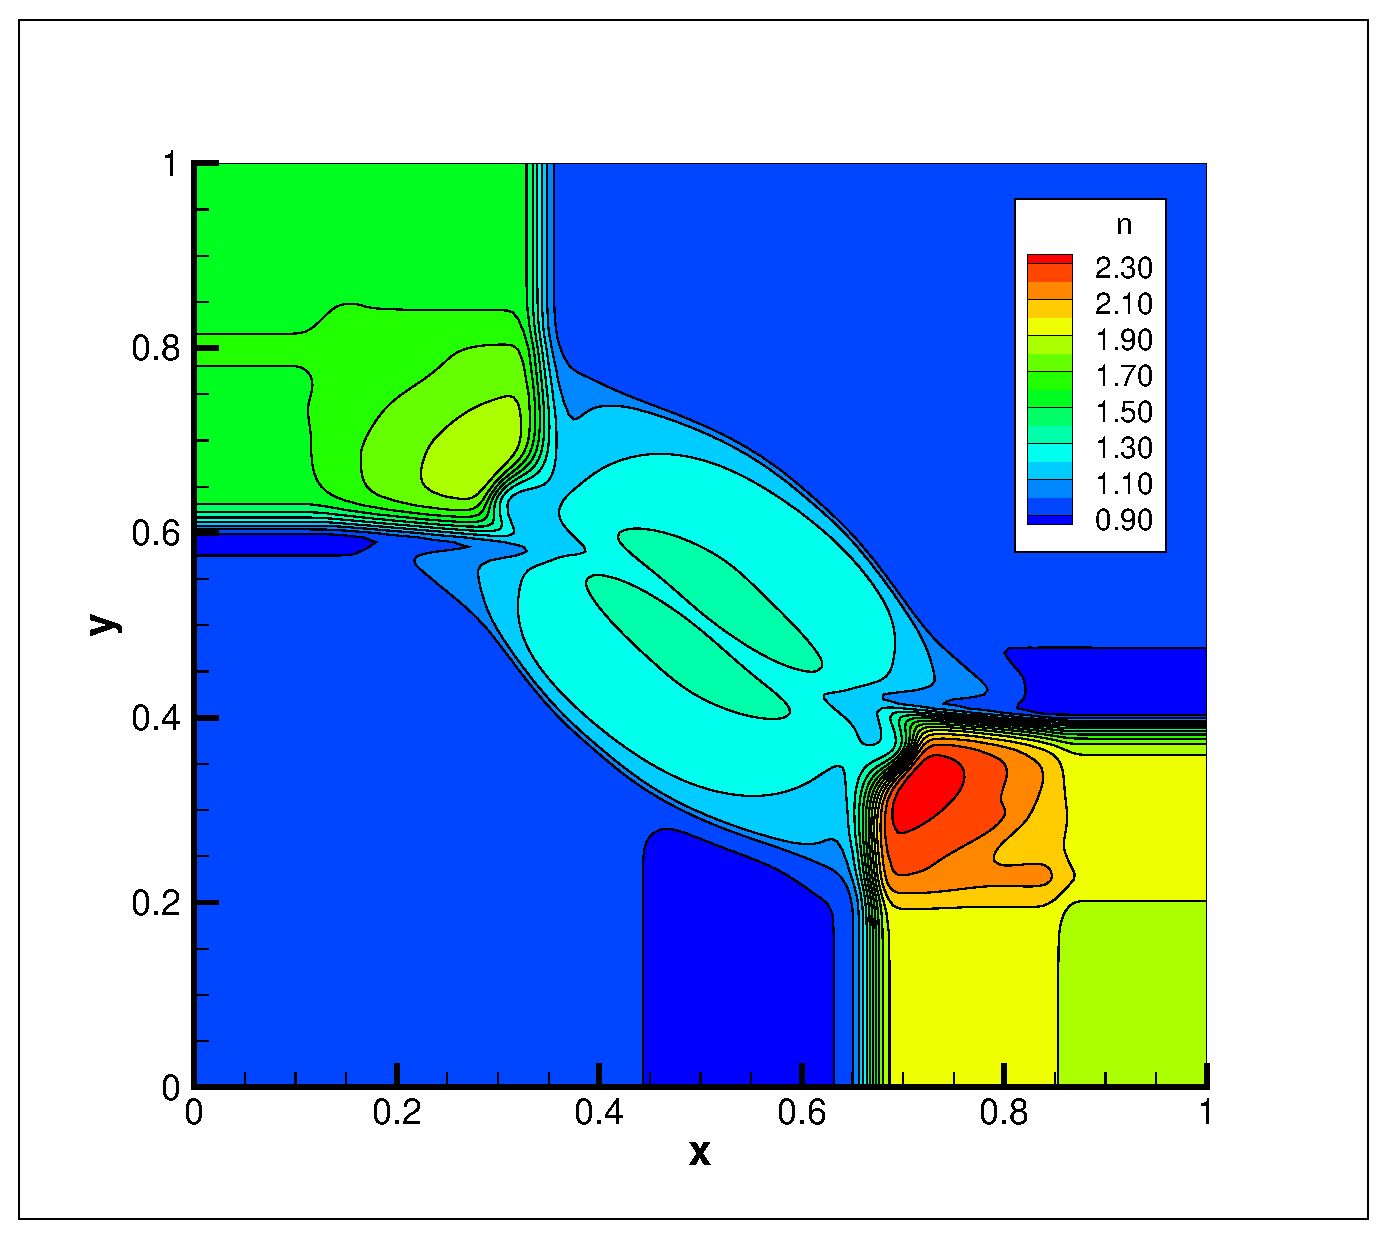
\includegraphics[trim = 20mm 15mm 20mm 20mm,clip,width=\textwidth]{ESBGK_MB_n}
                \caption{Number density (MB).}
                \label{fig:5ESBGK_MB_n}
        \end{subfigure}
        ~ %add desired spacing between images, e. g. ~, \quad, \qquad etc.
          %(or a blank line to force the subfigure onto a new line)
        \begin{subfigure}[b]{0.32\textwidth}
                \centering
                \includegraphics[trim = 20mm 15mm 20mm 20mm,clip,width=\textwidth]{ESBGK_MB_p}
                \caption{Pressure (MB). }
                \label{fig:5ESBGK_MB_p}
        \end{subfigure}
				~ %add desired spacing between images, e. g. ~, \quad, \qquad etc.
          %(or a blank line to force the subfigure onto a new line)
        \begin{subfigure}[b]{0.32\textwidth}
                \centering
                \includegraphics[trim = 20mm 15mm 20mm 20mm,clip,width=\textwidth]{ESBGK_MB_z}
                \caption{Fugacity (MB).}
                \label{fig:5ESBGK_MB_z}
        \end{subfigure}
        ~ %add desired spacing between images, e. g. ~, \quad, \qquad etc.
          %(or a blank line to force the subfigure onto a new line)
        \begin{subfigure}[b]{0.32\textwidth}
                \centering
                \includegraphics[trim = 20mm 15mm 20mm 20mm,clip,width=\textwidth]{ESBGK_FD_n}
                \caption{Number density (FD).}
                \label{fig:5ESBGK_FD_n}
        \end{subfigure}
        ~ %add desired spacing between images, e. g. ~, \quad, \qquad etc.
          %(or a blank line to force the subfigure onto a new line)
        \begin{subfigure}[b]{0.32\textwidth}
                \centering
                \includegraphics[trim = 20mm 15mm 20mm 20mm,clip,width=\textwidth]{ESBGK_FD_p}
                \caption{Pressure (FD).}
                \label{fig:5ESBGK_FD_p}
        \end{subfigure}
				~ %add desired spacing between images, e. g. ~, \quad, \qquad etc.
          %(or a blank line to force the subfigure onto a new line)
        \begin{subfigure}[b]{0.32\textwidth}
                \centering
                \includegraphics[trim = 20mm 15mm 20mm 20mm,clip,width=\textwidth]{ESBGK_FD_z}
                \caption{Fugacity (FD).}
                \label{fig:5ESBGK_FD_z}
        \end{subfigure}
				\caption{Comparison of results for \emph{Configuration 5} for three statistics using semiclassical ES equilibrium distribution with parameter $\it{b=0.5}$ and TVD method.}
				\label{fig:test_configuration5}
\end{figure}

In this configuration, shock, slip line, and rarefaction fan are conjectured to be propagating from interfaces of the four quadrants. A shock shall be seen propagating through quadrants 3 and 2, rarefaction fan through quadrants 4 and 1 and slip discontinuities through quadrants 2 and 1 and through quadrants 4 and 1. \\

We first report the results for the \emph{Configuration 5} for three statistics with parameter $b=0.5$. In Fig. \ref{fig:test_configuration5}, the number density, pressure and fugacity contours are shown for the three statistics at about the time instant similar to that reported in \cite{Laxliu95}\cite{schultzrinne}. From the density and pressure contours, one can identify the interesting and complicated wave patterns.   At the right top corner, the two slip lines $J_{21}$ and $J_{32}$ meet the sonic circle of the constant state in the second quadrant and continue as almost straight lines so that a quarter of the sonic circle lies in between.  Our results are consistent with calculations in \cite{Laxliu95}\cite{schultzrinne} and with the theoretical conjecture in \cite{ZhangZheng90} for the same configuration and with the same initial data.   There are detectable differences among the three statistics although the overall wave patterns are similar. Quantitatively, comparing the same contours for the three statistics, the numerical values of number density and pressure for the Bose-Einstein statistics are the largest among the three statistics and the Maxwell-Boltzmann statistics always lie between the other two as dictated by the $\theta$ values. \\

\begin{figure}
        \centering
        \begin{subfigure}[b]{0.32\textwidth}
                \centering
                \includegraphics[trim = 20mm 15mm 20mm 20mm,clip,width=\textwidth]{17ESBGK_BE_n}
                \caption{Number density (BE).}
                \label{fig:17ESBGK_BE_n}
        \end{subfigure}%
        ~ %add desired spacing between images, e. g. ~, \quad, \qquad etc.
          %(or a blank line to force the subfigure onto a new line)
        \begin{subfigure}[b]{0.32\textwidth}
                \centering
                \includegraphics[trim = 20mm 15mm 20mm 20mm,clip,width=\textwidth]{17ESBGK_BE_p}
                \caption{Pressure (BE).}
                \label{fig:17ESBGK_BE_p}
        \end{subfigure}
        ~ %add desired spacing between images, e. g. ~, \quad, \qquad etc.
          %(or a blank line to force the subfigure onto a new line)
        \begin{subfigure}[b]{0.32\textwidth}
                \centering
                \includegraphics[trim = 20mm 15mm 20mm 20mm,clip,width=\textwidth]{17ESBGK_BE_z}
                \caption{Fugacity (BE).}
                \label{fig:17ESBGK_BE_z}
        \end{subfigure}
				~ %add desired spacing between images, e. g. ~, \quad, \qquad etc.
          %(or a blank line to force the subfigure onto a new line)
        \begin{subfigure}[b]{0.32\textwidth}
                \centering
                \includegraphics[trim = 20mm 15mm 20mm 20mm,clip,width=\textwidth]{17ESBGK_MB_n}
                \caption{Number density (MB).}
                \label{fig:17ESBGK_MB_n}
        \end{subfigure}
        ~ %add desired spacing between images, e. g. ~, \quad, \qquad etc.
          %(or a blank line to force the subfigure onto a new line)
        \begin{subfigure}[b]{0.32\textwidth}
                \centering
                \includegraphics[trim = 20mm 15mm 20mm 20mm,clip,width=\textwidth]{17ESBGK_MB_p}
                \caption{Pressure (MB).}
                \label{fig:17ESBGK_MB_p}
        \end{subfigure}
				~ %add desired spacing between images, e. g. ~, \quad, \qquad etc.
          %(or a blank line to force the subfigure onto a new line)
        \begin{subfigure}[b]{0.32\textwidth}
                \centering
                \includegraphics[trim = 20mm 15mm 20mm 20mm,clip,width=\textwidth]{17ESBGK_MB_z}
                \caption{Fugacity (MB).}
                \label{fig:17ESBGK_MB_z}
        \end{subfigure}
        ~ %add desired spacing between images, e. g. ~, \quad, \qquad etc.
          %(or a blank line to force the subfigure onto a new line)
        \begin{subfigure}[b]{0.32\textwidth}
                \centering
                \includegraphics[trim = 20mm 15mm 20mm 20mm,clip,width=\textwidth]{17ESBGK_FD_n}
                \caption{Number density (FD).}
                \label{fig:17ESBGK_FD_n}
        \end{subfigure}
        ~ %add desired spacing between images, e. g. ~, \quad, \qquad etc.
          %(or a blank line to force the subfigure onto a new line)
        \begin{subfigure}[b]{0.32\textwidth}
                \centering
                \includegraphics[trim = 20mm 15mm 20mm 20mm,clip,width=\textwidth]{17ESBGK_FD_p}
                \caption{Pressure (FD).}
                \label{fig:17ESBGK_FD_p}
        \end{subfigure}
				~ %add desired spacing between images, e. g. ~, \quad, \qquad etc.
          %(or a blank line to force the subfigure onto a new line)
        \begin{subfigure}[b]{0.32\textwidth}
                \centering
                \includegraphics[trim = 20mm 15mm 20mm 20mm,clip,width=\textwidth]{17ESBGK_FD_z}
                \caption{Fugacity (FD).}
                \label{fig:17ESBGK_FD_z}
        \end{subfigure}
				\caption{Comparison of results for \emph{Configuration 17} for three statistics using ES equilibrium distribution with parameter $b=0.5$ and TVD method.}
				\label{fig:test_configuration17}
\end{figure}

Next, we report the results for \emph{Configuration 17}. The same contours of flow properties as in Fig. \ref{fig:test_configuration5} are shown in Fig. \ref{fig:test_configuration17}.  After some time, as shown in the figure, the two slip lines $J_{21}$ and $J_{34}$ part the wave patterns into a left and right part and connect with a vortex inside the subsonic region.
For the \emph{Configuration 17}, again, the wave patterns shown in Fig. \ref{fig:test_configuration17} are consistent with calculations in \cite{Laxliu95}\cite{schultzrinne} and  with the theoretical conjecture in \cite{ZhangZheng90} for the same configuration and with the same initial data.   Notable differences among the three statistics can be observed although the overall wave patterns are similar.  Quantitatively, the numerical values of number density and pressure contours for the Bose-Einstein statistics are the largest among the three statistics and the flow properties obtained by using Maxwell-Boltzmann statistics are always greater than those with obtained with Fermi-Dirac statistics and lower than those with Bose-Einstein statistics as it should be.

\subsection{Mesh refinement tests}
Here we investigate the consistency and convergence of our numerical implementation by increasing the number of grids in the computational domain and therefore reducing their size. Here we expect a decrease of the truncation error, and therefore observe converge pattern to the solution of the chosen configuration under test. We report in Fig. \ref{fig:Mesh_refinement} our findings in \emph{Configurations 5} and \emph{Configurations 17} using a grid $400\times400$, i.e. four times the total of cells used in our initial test grid. We observe in Figs. \ref{fig:400x400_FD_ESBGK_n} and \ref{fig:400x400_FD_ESBGK_p} that that slip line structures exhibit much sharper profiles with a refined mesh. This also true in the vicinity of rarefaction fans and contact discontinuities by observing structures in Figs. \ref{fig:400x400_FD_17ESBGK_n} and \ref{fig:400x400_FD_17ESBGK_p}. Both results in Fig. \ref{fig:Mesh_refinement} are computed with \emph{CFL} condition equal to 0.6 and corresponds to an output time of $t=0.25$. Most of our results here presented are obtained using a grid system $200\times200$ and they exhibit slightly smeared profiles compared to that using grid system $400\times400$ be completed.  The trend of grid convergence of the solutions can be clearly observed.

\begin{figure}
        \centering
        \begin{subfigure}[b]{0.45\textwidth}
                \centering
                \includegraphics[trim = 20mm 15mm 20mm 20mm,clip,width=\textwidth]{400x400_FD_ESBGK_n}
                \caption{Number density (FD) \\ ES model with $\it{b=0.5}$.}
                \label{fig:400x400_FD_ESBGK_n}
        \end{subfigure}%
				~ %add desired spacing between images, e. g. ~, \quad, \qquad etc.
          %(or a blank line to force the subfigure onto a new line)
				\begin{subfigure}[b]{0.45\textwidth}
                \centering
                \includegraphics[trim = 20mm 15mm 20mm 20mm,clip,width=\textwidth]{400x400_FD_ESBGK_p}
                \caption{Pressure (FD) \\ ES model with $\it{b=0.5}$.}
                \label{fig:400x400_FD_ESBGK_p}
        \end{subfigure}%
				 %add desired spacing between images, e. g. ~, \quad, \qquad etc.

					%(or a blank line to force the subfigure onto a new line)
					\begin{subfigure}[b]{0.45\textwidth}
                \centering
                \includegraphics[trim = 20mm 15mm 20mm 20mm,clip,width=\textwidth]{400x400_FD_17ESBGK_n}
                \caption{Number density (FD) \\ ES model with $\it{b=0.5}$.}
                \label{fig:400x400_FD_17ESBGK_n}
        \end{subfigure}%
				~ %add desired spacing between images, e. g. ~, \quad, \qquad etc.
          %(or a blank line to force the subfigure onto a new line)
				\begin{subfigure}[b]{0.45\textwidth}
                \centering
                \includegraphics[trim = 20mm 15mm 20mm 20mm,clip,width=\textwidth]{400x400_FD_17ESBGK_p}
                \caption{Pressure (FD) \\ ES model with $\it{b=0.5}$.}
                \label{fig:400x400_FD_17ESBGK_p}
        \end{subfigure}%
				\caption{Number density and pressure contours for \emph{Configuration 5} and \emph{Configuration 17} for a Fermi ideal gas using fine mesh.}
				\label{fig:Mesh_refinement}
\end{figure}

\subsection{Effect of parameter $\it{b}$ of ES equilibrium distribution on flow properties }

Here, we investigate quantitatively and qualitatively the effects of dimensionless parameter $\it{b}$ in the ellipsoidal statistical distribution model, $f^{ES}$, on the wave flow patterns and properties.  From qualitative observations on different configurations, it is shown that parameter $\it{b}$ influences the results by increasing or decreasing the sharpness of the profiles of every configurations. Quantitatively, we notice that it is not deterministic how this parameter may affect the overall magnitude of flow properties. We report this observations by using the number density contours for \emph{Configuration 5} evaluated with both quantum statistics in Fig. \ref{fig:test_b_parameter}.  We calculate three cases for the discrete values of $b=\{-0.5,\;0,\;0.75\}$; and the number density wave patterns for Bose-Einstein and Fermi-Dirac with $b=0.5$ are shown in Figs. \ref{fig:5ESBGK_BE_n} and \ref{fig:5ESBGK_FD_n}, respectively. Also it is noted that by setting $b=0$ we recover the traditional isotropic semiclassical equilibrium distribution, i.e., $f^{ES}= f^{eq}$.  By observing figures \ref{fig:5ESBGK_BE_n}, one can find differences in the density number contours and their numerical values, however, they are still consistent with calculations in \cite{Laxliu95}\cite{schultzrinne}.

\begin{figure}
        \centering
        \begin{subfigure}[b]{0.32\textwidth}
                \centering
                \includegraphics[trim = 20mm 15mm 20mm 20mm,clip,width=\textwidth]{ESBGK_BE_bn05_n}
                \caption{Density (BE) \\ ES model with $\it{b=-0.5}$.}
                \label{fig:ESBGK_BE_bn05_n}
        \end{subfigure}%
        ~ %add desired spacing between images, e. g. ~, \quad, \qquad etc.
          %(or a blank line to force the subfigure onto a new line)
        \begin{subfigure}[b]{0.32\textwidth}
                \centering
                \includegraphics[trim = 20mm 15mm 20mm 20mm,clip,width=\textwidth]{ESBGK_BE_b0_n}
                \caption{Density (BE) \\ ES model with $\it{b=0}$.}
                \label{fig:ESBGK_BE_b0_n}
        \end{subfigure}
        ~ %add desired spacing between images, e. g. ~, \quad, \qquad etc.
          %(or a blank line to force the subfigure onto a new line)
        \begin{subfigure}[b]{0.32\textwidth}
                \centering
                \includegraphics[trim = 20mm 15mm 20mm 20mm,clip,width=\textwidth]{ESBGK_BE_bp075_n}
                \caption{Density (BE) \\ ES model with $\it{b=0.75}$.}
                \label{fig:ESBGK_BE_bp075_n}
        \end{subfigure}
				~ %add desired spacing between images, e. g. ~, \quad, \qquad etc.
          %(or a blank line to force the subfigure onto a new line)
				\begin{subfigure}[b]{0.32\textwidth}
                \centering
                \includegraphics[trim = 20mm 15mm 20mm 20mm,clip,width=\textwidth]{ESBGK_FD_bn05_n}
                \caption{Density (FD) \\ ES model with $\it{b=-0.5}$.}
                \label{fig:ESBGK_FD_bn05_n}
        \end{subfigure}%
        ~ %add desired spacing between images, e. g. ~, \quad, \qquad etc.
          %(or a blank line to force the subfigure onto a new line)
        \begin{subfigure}[b]{0.32\textwidth}
                \centering
                \includegraphics[trim = 20mm 15mm 20mm 20mm,clip,width=\textwidth]{ESBGK_FD_b0_n}
                \caption{Density (FD) \\ ES model with $\it{b=0}$.}
                \label{fig:ESBGK_FD_b0_n}
        \end{subfigure}
        ~ %add desired spacing between images, e. g. ~, \quad, \qquad etc.
          %(or a blank line to force the subfigure onto a new line)
        \begin{subfigure}[b]{0.32\textwidth}
                \centering
                \includegraphics[trim = 20mm 15mm 20mm 20mm,clip,width=\textwidth]{ESBGK_FD_bp075_n}
                \caption{Density (FD) \\ ES model with $\it{b=0.75}$.}
                \label{fig:ESBGK_FD_bp075_n}
        \end{subfigure}	
        \caption{The effect of parameter $\it{b}$ on flow features for \emph{Configuration 5} for three statistics.}
				\label{fig:test_b_parameter}
\end{figure}
%The effect of parameter $b$ on the flow characteristics is also studied.  The results of number density contours for the Maxwell-Boltzmann statistics ($\theta=0$ in Eq. (\ref{eq:normalized_ESBGK_PDF})) for three values of $b$ are shown in Fig. 4.

\subsection{Observations on $W_{\alpha \beta}$ and pressure tensor components}
In Figs. \ref{fig:conf5_W_p_Tensor} \& \ref{fig:conf5_W_p_Tensor2} the contours of $W_{\alpha \beta}$ and $P_{\alpha \beta}$ tensor components of the ES model are depicted for \emph{Configuration 5} with $b=0.5$ using ideal gases following Bose-Einstein and Fermi-Dirac statistics, respectively. It is readily noticed that contours of diagonal tensor components, $W_{xx}$ and $W_{yy}$, are very similar but a closer look reveals that both differ slightly numerically. In contrast $W_{xy}$ component as depicted in Figs. \ref{fig:5ESBGK_BE_bp05_Wxy} and \ref{fig:5ESBGK_FD_bp05_Wxy} are numerically small compared to the former ones. However, this component contribution can not be neglected in the present anisotropic model. \\
By looking at pressure tensor components in Figs. \ref{fig:conf5_W_p_Tensor} \& \ref{fig:conf5_W_p_Tensor2}, it is evident that $W_{\alpha \beta}$ and $P_{\alpha \beta}$ tensor quantities are closely related. This was expected by recalling relations (\ref{eq:pressure_tensor_variables}), moreover, it is also easy to notice that the contribution of main diagonal tensor components generally will be greater than the rest of the tensor components. \\
Comparing the pressure components, as before, we observe that the main diagonal components, $P_{xx}$ and $P_{yy}$, exhibit similar flow patterns but again slight numerical differences can be identified.  Notice that the main diagonal components will be equal when the dimensionless parameter $\it{b = 0}$, i.e. $f^{eq}$ is used.  Based on the quantitative observations on several tested configurations, it is safe to conjecture that due to the slight differences on $P_{xx}$ \& $P_{yy}$ and the contribution of $P_{xy}$ components, as triggered by the dimensionless parameter $\it{b}$ of the ES distribution function, the anisotropic ES model contributes to relax the fixed Prandtl number condition of the traditional equilibrium distribution model, $f^{eq}$. \\
Notice the similar patterns between pressure contours in Figs. \ref{fig:conf5_W_p_Tensor} and \ref{fig:conf5_W_p_Tensor2}, the results also show that numerical pressure values are greater for Bose-Einstein statistics as expected.  Finally, although the kind of gas used in this examples are Bose and Fermi gases, the results are comparable to the earlier work of Lax \cite{Laxliu95} and \cite{schultzrinne} (classical gas) in terms of the expected flow patterns.

\begin{figure}
        \centering
        \begin{subfigure}[b]{0.32\textwidth}
                \centering
                \includegraphics[trim = 20mm 15mm 20mm 20mm,clip,width=\textwidth]{ESBGK_BE_bp05_Wxx}
                \caption{$W_{xx}$ (BE).}
                \label{fig:5ESBGK_BE_bp05_Wxx}
        \end{subfigure}%
        ~ %add desired spacing between images, e. g. ~, \quad, \qquad etc.
          %(or a blank line to force the subfigure onto a new line)
        \begin{subfigure}[b]{0.32\textwidth}
                \centering
                \includegraphics[trim = 20mm 15mm 20mm 20mm,clip,width=\textwidth]{ESBGK_BE_bp05_Wxy}
                \caption{$W_{xy}$ (BE).}
                \label{fig:5ESBGK_BE_bp05_Wxy}
        \end{subfigure}
        ~ %add desired spacing between images, e. g. ~, \quad, \qquad etc.
          %(or a blank line to force the subfigure onto a new line)
        \begin{subfigure}[b]{0.32\textwidth}
                \centering
                \includegraphics[trim = 20mm 15mm 20mm 20mm,clip,width=\textwidth]{ESBGK_BE_bp05_Wyy}
                \caption{$W_{yy}$ (BE).}
                \label{fig:5ESBGK_BE_bp05_Wyy}
        \end{subfigure}
				~ %add desired spacing between images, e. g. ~, \quad, \qquad etc.
          %(or a blank line to force the subfigure onto a new line)
				\begin{subfigure}[b]{0.32\textwidth}
                \centering
                \includegraphics[trim = 20mm 15mm 20mm 20mm,clip,width=\textwidth]{ESBGK_BE_pxx}
                \caption{$P_{xx}$ (BE).}
                \label{fig:ESBGK_BE_pxx}
        \end{subfigure}%
        ~ %add desired spacing between images, e. g. ~, \quad, \qquad etc.
          %(or a blank line to force the subfigure onto a new line)
        \begin{subfigure}[b]{0.32\textwidth}
                \centering
                \includegraphics[trim = 20mm 15mm 20mm 20mm,clip,width=\textwidth]{ESBGK_BE_pxy}
                \caption{$P_{xy}$ (BE).}
                \label{fig:ESBGK_BE_pxy}
        \end{subfigure}
        ~ %add desired spacing between images, e. g. ~, \quad, \qquad etc.
          %(or a blank line to force the subfigure onto a new line)
        \begin{subfigure}[b]{0.32\textwidth}
                \centering
                \includegraphics[trim = 20mm 15mm 20mm 20mm,clip,width=\textwidth]{ESBGK_BE_pyy}
                \caption{$P_{yy}$ (BE).}
                \label{fig:ESBGK_BE_pyy}
        \end{subfigure}
        \caption{$W_{\alpha \beta}$ \& $P_{\alpha \beta}$ components of \emph{Configuration 5} using ES model for Bose-Einstein statistics with $\it{b=0.5}$.}
				\label{fig:conf5_W_p_Tensor}
\end{figure}

\begin{figure}
        \centering
        \begin{subfigure}[b]{0.32\textwidth}
                \centering
                \includegraphics[trim = 20mm 15mm 20mm 20mm,clip,width=\textwidth]{ESBGK_FD_bp05_Wxx}
                \caption{$W_{xx}$ (FD).}
                \label{fig:5ESBGK_FD_bp05_Wxx}
        \end{subfigure}%
        ~ %add desired spacing between images, e. g. ~, \quad, \qquad etc.
          %(or a blank line to force the subfigure onto a new line)
        \begin{subfigure}[b]{0.32\textwidth}
                \centering
                \includegraphics[trim = 20mm 15mm 20mm 20mm,clip,width=\textwidth]{ESBGK_FD_bp05_Wxy}
                \caption{$W_{xy}$ (FD).}
                \label{fig:5ESBGK_FD_bp05_Wxy}
        \end{subfigure}
        ~ %add desired spacing between images, e. g. ~, \quad, \qquad etc.
          %(or a blank line to force the subfigure onto a new line)
        \begin{subfigure}[b]{0.32\textwidth}
                \centering
                \includegraphics[trim = 20mm 15mm 20mm 20mm,clip,width=\textwidth]{ESBGK_FD_bp05_Wyy}
                \caption{$W_{yy}$ (FD).}
                \label{fig:5ESBGK_FD_bp05_Wyy}
        \end{subfigure}
				~ %add desired spacing between images, e. g. ~, \quad, \qquad etc.
          %(or a blank line to force the subfigure onto a new line)
				\begin{subfigure}[b]{0.32\textwidth}
                \centering
                \includegraphics[trim = 20mm 15mm 20mm 20mm,clip,width=\textwidth]{ESBGK_FD_pxx}
                \caption{$P_{xx}$ (FD).}
                \label{fig:ESBGK_FD_pxx}
        \end{subfigure}%
        ~ %add desired spacing between images, e. g. ~, \quad, \qquad etc.
          %(or a blank line to force the subfigure onto a new line)
        \begin{subfigure}[b]{0.32\textwidth}
                \centering
                \includegraphics[trim = 20mm 15mm 20mm 20mm,clip,width=\textwidth]{ESBGK_FD_pxy}
                \caption{$P_{xy}$ (FD).}
                \label{fig:ESBGK_FD_pxy}
        \end{subfigure}
        ~ %add desired spacing between images, e. g. ~, \quad, \qquad etc.
          %(or a blank line to force the subfigure onto a new line)
        \begin{subfigure}[b]{0.32\textwidth}
                \centering
                \includegraphics[trim = 20mm 15mm 20mm 20mm,clip,width=\textwidth]{ESBGK_FD_pyy}
                \caption{$P_{yy}$ (FD).}
                \label{fig:ESBGK_FD_pyy}
        \end{subfigure}
        \caption{$W_{\alpha \beta}$ \& $P_{\alpha \beta}$ components of \emph{Configuration 5} using ES model for Fermi-Dirac statistics with $\it{b=0.5}$.}
				\label{fig:conf5_W_p_Tensor2}
\end{figure}

\section{Concluding Remarks}
\label{remarks}
The semiclassical ellipsoidal statistical equilibrium distribution of Wu et al. \cite{Wu2012} has been derived through maximum entropy principle and conserves the mass, momentum and energy but differs from the standard Bose-Einstein or Fermi-Dirac distribution. This ES distribution is anisotropic thus it can possess additional high order moments, therefore, its gas dynamical features are not well known and are worth exploring. In this work, the unsteady quantum gas dynamical flow features as dictated by the semiclassical ellipsoidal statistical equilibrium distribution is numerically studied.  The computational method treats the governing equation in phase space and employs the discrete ordinate method and high resolution shock capturing schemes. Specifically, we describe the solution method in details for the equation in two space dimensions.   A decoding procedure is devised for the semiclassical ellipsoidal statistical distribution which is different from that for standard Bose-Einstein or Fermi-Dirac distribution.  Computations of two-dimensional Riemann problems for gas flows of arbitrary particle statistics are presented and all our results are in good agreement with the calculations in \cite{Laxliu95}\cite{schultzrinne} and consistent with the theoretical conjecture in \cite{ZhangZheng90}.  The effect of the parameter $\it{b}$ of the ES model is studied.  Results showed how this parameter interacts with the pressure tensor and this can influence the Prandtl number in the non-equilibrium flows and therefore the transport properties of classical and quantum gases when the full semiclassical Boltzmann-ES-BGK equation is considered. These computational examples serve the purpose of exploring the nonlinear manifestation of shock wave, contact line and rarefaction wave and testing the robustness of the present method. All the expected flow profiles comprising shock, rarefaction wave and contact discontinuities of semiclassical ideal gases and their nonlinear interactions can be observed with considerably good detail and are in consistency with available results. The present work emphasizes on building the unified and parallel framework for treating semiclassical gas dynamics of three statistics. Extensions to three space dimensions and more complex geometries in general coordinates are straightforward and can be done following the same framework presented here.

\section{Acknowledgement*}
\label{Acknowledgements}

This work is done under the auspices of National Science Council, TAIWAN through grants NSC-99-2221-E002-084MY3, NSC-100-2221-E002-106MY3 and CASTS 10R80909-4.

%% The Appendices part is started with the command \appendix;
%% appendix sections are then done as normal sections
%% \appendix

%%%%%%%%%% Insert bibliography here %%%%%%%%%%%%%%

\bibliographystyle{prsb}
\bibliography{SB-ESBGK}

\end{document} 